\documentclass{standalone}
\usepackage{tikz}
\usetikzlibrary{shapes.misc}
\usetikzlibrary{arrows,positioning} 
\tikzset{
    %Define standard arrow tip
    >=stealth',
    %Define style for boxes
    punkt/.style={
           circle,
           draw = black, very thick,
           text centered, 
           minimum height = 3em},
    snpt/.style={
    	   circle,
    	   draw = black, very thick,
    	   text centered},
    % Define arrow style
    ests/.style={
           ->,
           thick},
    plt/.style={
           ->, blue, dashed,
           thick},
    dts/.style={
           ->, dotted,
           thick},
    dtts/.style={
           ->, dashed,
           thick}
}

\begin{document}
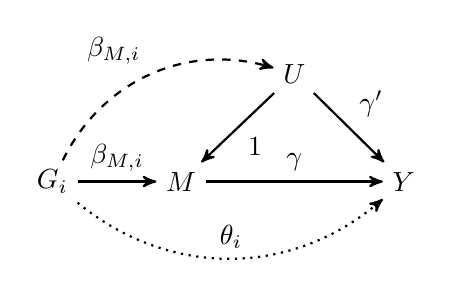
\begin{tikzpicture}[node distance=1cm, auto]
 %nodes
\node (Y) {$Y$};
\node[left=of Y] (dummy){};
\node[left=of dummy] (M) {$M$}
	edge[ests] node {$\gamma$} (Y);
\node [above = of dummy] (U) {$U$}
	edge[ests] node {1} (M)
	edge[ests] node {$\gamma^{\prime}$} (Y);
\node [left = of M] (G) {$G_i$}
	edge[ests] node {$\beta_{M,i}$} (M)
	edge[dtts, bend left = 40] node {$\beta_{M,i}$} (U)
	edge[dts, bend right=40]  node {$\theta_i$} (Y);
\end{tikzpicture}
\end{document}

